\newpage
\section{Capitulo I}
\section*{Generalidades de la empresa}
En este primer capitulo, se proporciona un análisis detallado de las generalidades de la empresa. Se examinaran aspectos clave como su razón social, RUC, y gerencia, así como su misión, visión y valores fundamentales que guían su operación. Además se describirán los servicios ofrecidos por la empresa, el mercado en el que opera y los clientes principales a los que se dirige.
\subsection{1.1 Razón social}
En esta sección se proporciona la información general de la empresa, como la gerencia; razón social; dirección; ruc; principal actividad económica; logo y ubicación.
\begin{itemize}
    \item[] \textbf{GERENTE GENERAL: }CARCAUSTO HUACHANI GUSTAVO ADOLFO
    \item[] \textbf{RAZÓN SOCIAL: } AUTOMOTRIZ PELAYO S.A.C.
    \item[] \textbf{DIRECCION: } MERCURIO MZA. K LOTE. 3 CAMPO MARTE ZONA A AREQUIPA - AREQUIPA - PAUCARPATA
    \item[] \textbf{RUC:} 20605004726    
    \item[] \textbf{ACTIVIDAD ECONÓMICA: }MANTENIMIENTO Y REPARACIÓN DE VEHÍCULOS AUTOMOTORES
\end{itemize}
\begin{figure}[h]
    \centering
        \captionsetup{singlelinecheck=false}
    \caption*{Logo de la Empresa}
    
\includegraphics[width=5cm]{imagenes/logo.png}
    \label{fig:logo}
\end{figure}
\newpage

\subsection{1.2 Misión, Visión, Objetivos, Valores de la empresa}
Esta sección proporciona una comprensión de la dirección y los principios fundamentales de la empresa, a través de la misión se destaca su compromiso con el mejor desenvolvimiento en su rubro, mientras la visión enfatiza su aspiración de liderazgo en el sector. Los objetivos establecen las metas especifícas para su mejora en la atención al cliente, y los valores fundamentales que guían las acciones de la empresa.
\subsubsection*{1.2.1 Misión}
Nos dedicamos a proporcionar servicios de mantenimiento mecánico de primera calidad para una amplia variedad de vehículos y maquinaria. Nuestro compromiso es superar constantemente las expectativas de nuestros clientes, ofreciendo soluciones integrales, confiables y eficientes. Además, nos comprometemos a promover un ambiente de trabajo seguro, colaborativo y profesional para nuestro equipo, fomentando el crecimiento personal y profesional de nuestros empleados.
\subsubsection*{1.2.2 Visión}
Buscamos ser reconocidos como líderes en el sector automotriz y de mantenimiento mecánico, Buscamos destacarnos no solo por nuestra excelencia en el servicio al cliente, sino también por nuestro firme compromiso con la innovación y la mejora continua. Aspiramos a inspirar confianza y seguridad en cada interacción con nuestros clientes.


\subsubsection*{1.2.3 Objetivos de la Empresa}
%Explicar
Los objetivos de la empresa son metas específicas que guían la dirección estratégica y orientan sus acciones hacia los resultados deseados. Representan los logros cuantitativos y cualitativos que la empresa busca alcanzar en un período determinado, proporcionando un marco para la toma de decisiones y la asignación de recursos. Estos objetivos son fundamentales para establecer una visión clara del camino hacia el éxito y para medir el progreso de la empresa en su conjunto.


\paragraph{Objetivo Principal. }Incrementar la satisfacción y el numero de clientes, así como la rentabilidad de la empresa.
\paragraph{Objetivos Secundarios. }Los siguientes objetivos secundarios desglosan el objetivo principal en áreas clave como la expansión de la clientela, la mejora operativa y la calidad del servicio, asegurando que cada aspecto contribuya al éxito y satisfacción del cliente.
\begin{itemize}
    \item Ampliar la cartera de clientes aumentando el número de clientes durante el próximo trimestre.
    \item Mejorar la eficiencia operativa reduciendo tiempos de espera mediante la optimización de los procesos operativos.
    \item Mejorar la calidad de servicios ofrecidos.
\end{itemize}

\subsubsection*{1.2.4 Valores de la Empresa}
%Explicar 
Los valores de una empresa son principios éticos fundamentales que establecen la cultura de la organización y permiten crear pautas de comportamiento coherentes. En el caso de AUTOMOTRIZ PELAYO S.A.C., los valores centrales que guían todas las operaciones y decisiones son:
\begin{enumerate}
    \item Calidad: Compromiso con la excelencia en la ejecución de cada servicio, asegurando la máxima calidad en cada tarea realizada.
    \item Integridad: Actuar con honestidad, transparencia y ética en todas las interacciones con clientes, empleados y socios comerciales.
    \item Compromiso con el cliente: Priorizar las necesidades y la satisfacción del cliente, ofreciendo soluciones personalizadas y un servicio excepcional.
    \item Profesionalismo: Actuar con responsabilidad y diligencia en cada tarea.
    \item Seguridad: Priorizar la seguridad de los empleados y clientes en todas las operaciones y actividades de la empresa.
\end{enumerate}
\subsection{1.3 Servicios, mercado, clientes}
La siguiente sección abordará los servicios ofrecidos por AUTOMOTRIZ PELAYO S.A.C., así como el mercado al que se dirige y sus principales clientes. En cuanto a los servicios, se proporcionará un detalle de las distintas categorías de mantenimiento y reparación mecánica ofrecidos. Se explicará cómo estos servicios contribuyen a satisfacer las necesidades de los clientes. Además, se analizará el mercado local en el que opera la empresa. Se describirá el contexto del mercado de servicios de mantenimiento mecánico y reparación de vehículos y maquinaria. Finalmente, se identificarán los principales clientes de la empresa, clasificándolos en clientes privados e industriales.

\subsubsection*{1.3.1 Servicios}
AUTOMOTRIZ PELAYO S.A.C. ofrece una gama completa de servicios de mantenimiento y reparación mecánica, diseñados para satisfacer las diversas necesidades de sus clientes. La empresa se especializa en el cuidado y mantenimiento de vehículos y maquinaria, brindando soluciones integrales que aseguran un rendimiento óptimo y prolongan la vida útil de los equipos. A continuación, se detalla la oferta de servicios, dividida en dos categorías principales: mantenimiento mecánico y reparación.

\paragraph{Servicios de Mantenimiento Mecánico. }Estos servicios están diseñados para mantener los vehículos y maquinaria en condiciones óptimas de funcionamiento y prevenir posibles fallos. Incluyen una serie de acciones preventivas que ayudan a identificar y corregir problemas antes de que se conviertan en averías mayores, asegurando así una mayor eficiencia y seguridad operativa: 
\begin{itemize}
    \item Mantenimiento preventivo para vehículos y maquinaria.
    \item Cambios de aceite y filtros.
    \item Lubricación de piezas y componentes.
    \item Servicios de diagnóstico y revisión periódica.
\end{itemize}
\paragraph{Servicios de Reparación. }AUTOMOTRIZ PELAYO S.A.C. ofrece una serie de servicios de reparación para corregir y solucionar problemas mecánicos y eléctricos en vehículos y maquinaria. Estos servicios están destinados a restablecer el funcionamiento normal y seguro de los equipos, incluyendo reparaciones específicas y la sustitución de componentes defectuosos, así como la restauración de la estructura y la estética de los vehículos.
\begin{itemize}
    \item Reparación de sistemas mecánicos y eléctricos de vehículos y maquinaria.
    \item Sustitución de piezas y componentes defectuosos.
    \item Solución de problemas específicos o averías.
    \item Reparación de daños estructurales.
    \item Servicios de pintura y restauración
\end{itemize}

\subsubsection*{1.3.2 Mercado}
%La empresa AUTOMOTRIZ PELAYO S.A.C. opera en el mercado local de servicios de mantenimiento mecánico y reparación de vehículos y maquinaria en la región de Arequipa.
AUTOMOTRIZ PELAYO S.A.C. opera en el mercado local de servicios de mantenimiento mecánico y reparación de vehículos y maquinaria en la región de Arequipa. Este mercado está compuesto principalmente por consumidores y empresas de la región que requieren servicios especializados para el mantenimiento y la reparación de sus vehículos. La empresa se enfoca en satisfacer la demanda, ofreciendo soluciones adaptadas a las necesidades específicas de los clientes en la zona, lo que le permite competir eficazmente en un entorno donde la proximidad y la calidad del servicio son cruciales para el éxito.


\subsubsection*{1.3.3 Clientes Principales}
Identificar y comprender a los principales clientes de AUTOMOTRIZ PELAYO S.A.C. es clave para desarrollar estrategias que respondan efectivamente a sus necesidades. Los clientes de la empresa se dividen en dos categorías principales: clientes privados e industriales, cada uno con características y requisitos específicos que la empresa busca satisfacer mediante sus servicios especializados:

\paragraph{Clientes Privados. }Los clientes privados de AUTOMOTRIZ PELAYO S.A.C. son individuos que poseen vehículos particulares y requieren servicios de mantenimiento y reparación para mantener sus automóviles en óptimas condiciones. Estos clientes buscan soluciones confiables y de calidad para garantizar la seguridad y el buen funcionamiento de sus vehículos. La empresa se compromete a ofrecer un servicio personalizado y eficiente que satisfaga las expectativas de cada propietario de vehículo.
 
\begin{itemize}
    \item Propietarios de vehículos particulares: Estos clientes son propietarios individuales de vehículos que requieren servicios de mantenimiento y reparación para sus automóviles personales.
\end{itemize}

\paragraph{Clientes Industriales. }Los clientes industriales de AUTOMOTRIZ PELAYO S.A.C. incluyen empresas que poseen flotas de vehículos o maquinaria pesada y requieren servicios de mantenimiento y reparación para garantizar la continuidad y eficiencia de sus operaciones. Estos clientes valoran la capacidad de la empresa para manejar servicios complejos y su habilidad para ofrecer soluciones a medida que aseguren la operatividad y longevidad de sus equipos.

\begin{itemize}
    \item Empresas de transporte: Incluye empresas dedicadas al transporte de mercancías o pasajeros que requieren servicios de mantenimiento y reparación para su flota de vehículos comerciales. 
    \item Empresas industriales con maquinaria: Comprende empresas que operan maquinaria industrial y requieren servicios de mantenimiento mecánico para garantizar el funcionamiento óptimo de sus equipos.
    \item Talleres mecánicos: Otros talleres mecánicos pueden subcontratar servicios especializados a AUTOMOTRIZ PELAYO S.A.C. cuando enfrentan tareas que están fuera de su experiencia o capacidad. 
\end{itemize}

%Estructura 
\subsection{1.4 Estructura de la Organización}
La estructura de la organización define técnicamente las relaciones que deben existir entre las funciones, niveles y actividades de las personas con el fin de lograr máxima eficiencia en la realización de planes y objetivos.
En la parte superior de este organigrama se encuentra el gerente general, quien está a cargo de la gestión global de la empresa. Bajo el gerente general, se encuentra el gerente de sucursal, este asu vez lidera la sucursal de la empresa. A su vez, el gerente de sucursal supervisa a un técnico, quien es responsable de llevar a cabo las actividades técnicas y operativas en su respectiva sucursal. Esta organizacion se repite en cada una de las 3 sucursales que tiene la empresa.

%\begin{figure}[H]
%    \centering
%    \caption{Organigrama de la empresa}
%    \label{organigrama}
%    \includesvg[width=15cm]{imagenes/Organigrama.svg}
%\end{figure}

\begin{figure}[H]
    \centering
    \caption{Organigrama de la empresa}
    \label{organigrama}
    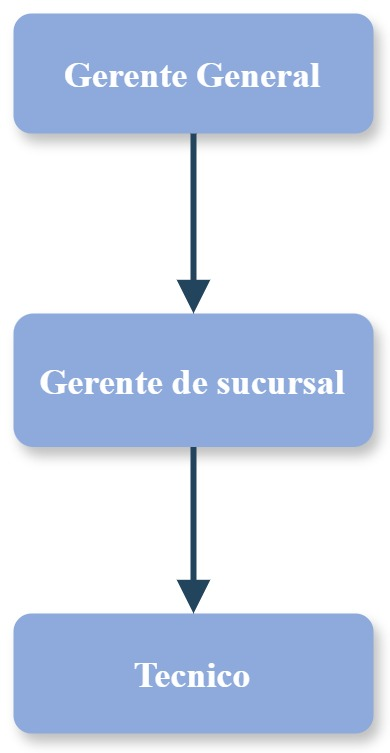
\includegraphics[width=6cm, height=10cm]{imagenes/cap1/Organigrama123.jpg}
\end{figure}

\subsection{1.5 Otra información relevante de la empresa donde se desarrolla el proyecto.}
La empresa Automotriz PELAYO S.A.C. se estableció en el año 2019 fundada por el Sr. Gustavo Adolfo Carcausto Huachani, con una amplia experiencia trabajando en varios talleres, hasta que decidió emprender su propio negocio.
Actualmente, la empresa ha demostrado un compromiso constante con la excelencia en el servicio al cliente y la calidad en sus operaciones. Además se enorgullece de mantener relaciones sólidas con proveedores de repuestos y materiales de alta calidad, garantizando así la fiabilidad y durabilidad de sus servicios.
El Gerente General sostiene que como empresa automotriz, su objetivo es satisfacer los requerimientos y expectativas de los clientes, gestionando eficientemente los recursos y procesos. Además, buscan prevenir incidentes, enfermedades ocupacionales, impactos ambientales y conflictos sociales, promoviendo una cultura de seguridad y mantenibilidad. También se comprometen a cumplir con la legislación nacional y normas vigentes relacionadas con la calidad, seguridad, salud, ambiental y social aplicables a sus operaciones.
